%%%%%%%%%%%%%%%%%%%%%%%%%%%%%% -*- Mode: Latex -*- %%%%%%%%%%%%%%%%%%%%%%%%%%%%
%% main.tex<fourier_decomp> -- 
%% Last Modified On: Thu Apr 13 16:15:17 2023 (+0200)
%%%%%%%%%%%%%%%%%%%%%%%%%%%%%%%%%%%%%%%%%%%%%%%%%%%%%%%%%%%%%%%%%%%%%%%%%%%%%%%

\documentclass{zamarep}

% Useful LaTeX packages
\usepackage{mathtools}
\usepackage{mathcalbd} % for \pol macro

\usepackage[colorlinks]{hyperref} % should be loaded last
\usepackage{cleveref}  % should be loaded last last

\title{Incrementally Verifiable Computation and Verifiable FHE}
\subtitle{Feasibility and Applicability}

\author[MW]{Michael Walter}

% \date{April 13, 2023}

%\titlegraphic[credit={Erik Karits}]{%
%  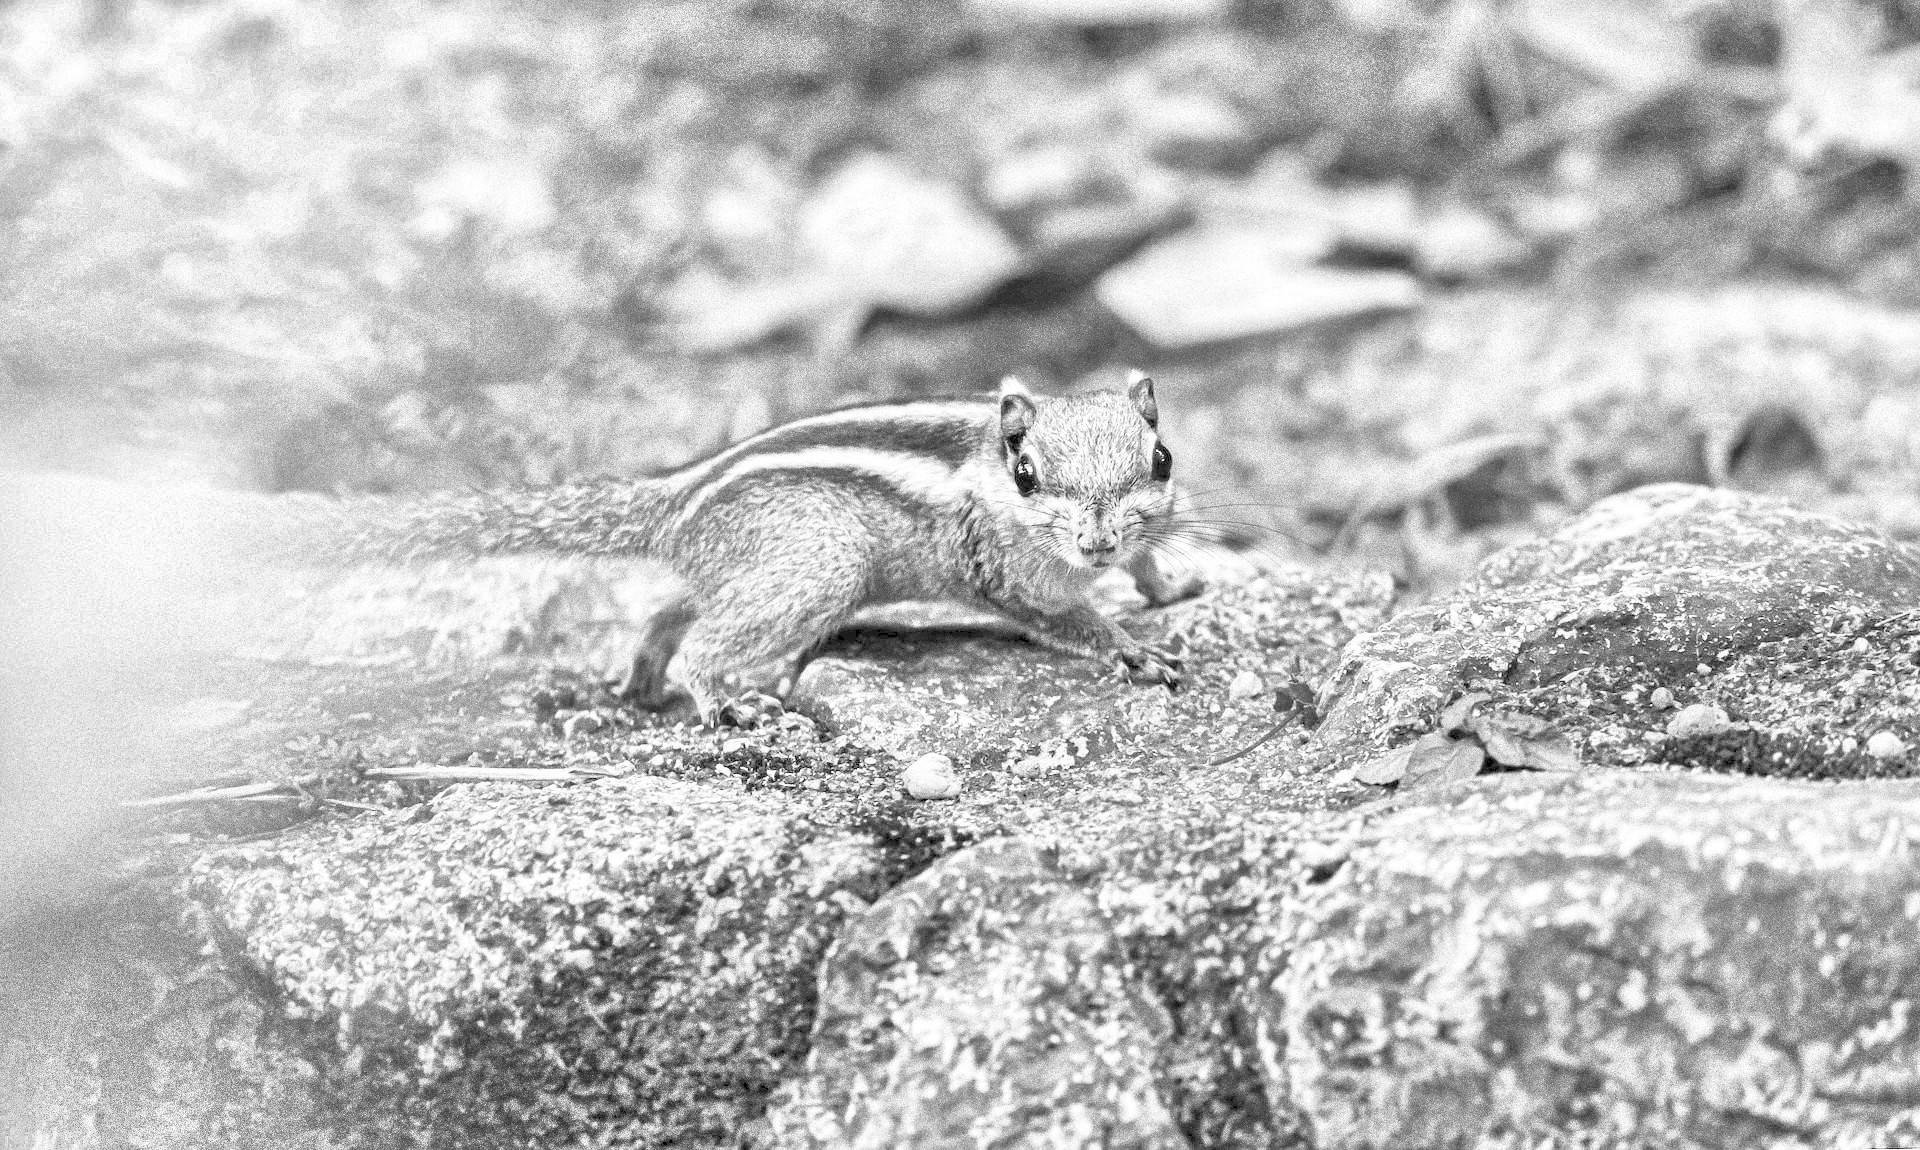
\includegraphics{erik-karits-Ivy_nqt6gTc-unsplash}}


% --- Macros
% \newcommand{\ints}{\mathds{Z}}
% \newcommand{\reals}{\mathds{R}}
% \newcommand{\torus}{\mathds{T}}
% \newcommand*{\pol}{\mathcalbd}
% \newcommand*{\SQ}{\mathit{S\!Q}}

\newcommand{\field}{\mathbb{F}}
\newcommand{\sha}{\texttt{SHA256}~}
% \newcommand{\rs}[3]{\mathrm{RS()}}
\newcommand{\abs}[1]{\lvert #1 \rvert}
\newcommand{\Sel}[1]{S_{\mathrm{#1}}}
\newcommand{\psel}[1]{p_{\mathrm{#1}}}

\begin{document}

\maketitle


%%%%%%%%%%%%%%%%%%%%%%%%%%%%%%%%%%%%%%%%%%%%%%%%%%%%%%%%%%%%%%%%%%%%%%%%%%%%%%% 
\section{Introduction}\label{sec:introduction}
%%%%%%%%%%%%%%%%%%%%%%%%%%%%%%%%%%%%%%%%%%%%%%%%%%%%%%%%%%%%%%%%%%%%%%%%%%%%%%% 
This document is part of our effort to develop a SNARK prototype that is able to prove the correctness of a PBS evaluation in reasonable time. For an overview of our approach we refer to \cite{part1,part2}. In this document we evaluate the practicality of applying Incrementally Verifiable Computation (IVC) to prove the correct evaluation of the blind rotation.

\section{Incrementally Verifiable Computation}
\label{sec:ivc}

The concept of IVC goes back to the work of \cite{TCC:Valiant08}. The idea is to prove the correctness of a long computation step by step and be able to verify this computation at any intermediate point, even before the entire computation is completed. Since most SNARKs prove computation in the circuit model, one may also think of IVC as a way to prove loops more efficiently than rolling out the entire loop into a large circuit. This is particularly useful when the prover time is super-linear as it allows to break up the proof of the large circuit of size $nC$ into $n$ proofs for small circuits of size $C$. In our setting, we target the blind rotation for the application of IVC as it is essentially a large loop. 

In the literature, there are two main approaches discussed to achieve IVC, one based on recursive proofs and one based on folding. We will describe the high level idea of each of them below and then discuss their advantages and disadvantages for our setting.

\section{Recursion}
\label{sec:recurse}

The concept of recursion is based on the observation that the computation of the verifier is just a circuit that can be the input to a SNARK itself. So after evaluating a given circuit, the prover may generate the proof for the circuit using the SNARK and then either send this proof directly, or prove knowledge of the proof by evaluating and proving the verifier circuit. Note that the two SNARKs applied here do not necessarily have to be the same, so the prototypical application of recursion is to combine the best properties of two different SNARKs.

In our setting, we are more interested in using recursion in order to prove a loop, i.e. IVC. Let $F$ be the function describing the step function of the loop, i.e.\ we want to proof $y = F^{n}(x)$, where $F^{n}(x)$ corresponds to applying $F$ successively $n$ times to $x$. We may augment $F$ to obtain a function $F'$ that takes as input a value $y_i$ and a proof $\pi_i$ and outputs $y_{i+1}$ and a proof $\pi_{i+1}$ attesting to the correctness of the statement:
\begin{itemize}
\item $y_{i+1} = F(y_i)$ and
\item the verifier accepts $\pi_i$ as a proof of $y_{i} = F(x)$.
\end{itemize}
The prover may now successively evaluate $(y_i, \pi_i) = F'(y_{i-1}, \pi_{i-1})$ and obtain the output $y_{n}$ along with a succinct proof $\pi_{n}$.

While this approach allows to transform the problem of proving the computation of $F^n$ to $n$ computations of $F'$, there is some overhead due to the fact that we prove $F'$ instead of $F$ for each step of the computation, meaning the circuit size for each step increased. This increase essentially corresponds to the size of the verifier circuit, which in turn depends on the used SNARK. In our setting, we use a FRI based PCS, which has a relatively large verifier circuit, but on the other hand avoids the need of cycles of elleptic curves plaguing other approaches.


\section{Folding}
\label{sec:fold}

The folding paradigm was more recently introduced in the work of \cite{EPRINT:BowGriHop19} and has spurred a flurry of new works \cite{C:KotSetTzi22,EPRINT:KotSet22,cryptoeprint:2023/620,C:BCLMS21,TCC:BCMS20,sangria}. Recall that SNARKs are constructed by arithmetizing the computation to turn it into some intermediate format, e.g. R1CS or PLONK, which is then combined with a suitable polynomial commitment scheme. The intermediate format is some type of mathematical object (hence the term \emph{arithmetization}), e.g. a contraint system or a polynomial, with specific properties that ensure that the computation is correct and allow to prove these properties. In the following we will denote a computation in the intermediate format by an \emph{instance}. The general idea of a folding scheme is to take two instances of similar size and merge them into one instance of the same size. By using randomness provided by the verifier, the key observation is that the merged instance is with high probability not going to be a valid instance if one of the two initial instances was not valid. In turn that means that it is sufficient to prove the merged instance in order to ensure that the two initial instances were correct. 

Note that such an approach allows to prove loops by constructing an instance for each loop iteration and successively folding them together into an instance of size comparable to one loop iteration. Finally, the idea is to apply the proof only to the merged instance.

In contrast to IVC based on recursion, folding schemes do not require to compute an entire proof for each loop iteration --- it is sufficient to compute the arithmetization of each step. Accordingly, this has the potential of being significantly more efficient than the approach based on recursion. On the other hand, folding does have its drawbacks, mostly hidden by the drastically simplified description above. In particular, it introduces cross terms (or error terms) that need to be handled. This requires to relax the conditions on the instances, introduces homomorphic commitments that need to be included in the circuit, and generally complicates the method significantly.

\section{Discussion}
\label{sec:dis}

In principle, both approaches seem to bear the potential of reducing the cost of proving the blind rotation. IVC based on recursion might be less efficient, but the concept has been known for a longer time and thus is more mature. In particular, there are efficient implementations of recursive SNARKs, for example plonky2 \cite{plonky2}, which is implemented in Rust and shares many properties of our prototype (a SNARK based on PLONK and FRI), but is optimized for recursion. Although documentation is scarce, preliminary experimentation suggests that it should be possible to realize an IVC-based blind rotation using plonky2, which has the potential to obtain results in a relatively short timeframe.

On the other hand, IVC based on folding seems to be more promising with regards to performance, but, as far as we know, there is at this point only one implementation of a folding scheme, namely Nova \cite{nova,C:KotSetTzi22}. Nova diverges significantly from our current approach by using the R1CS arithmetization. So if we wanted to continue our current approach based on PLONK, we would presumably have to implement the folding scheme ourselves, which will likely be more time consuming than using an efficient implementation like plonky2.

In summary, the approach based on recursion promises concrete results in the short term, while the one based on folding is likely to produce better results in the long term. Accordingly, we plan on exploring folding further in the near future with the goal of including an implementation in our prototype. 


% --- Bibliography
\bibliographystyle{alphaurl}
\bibliography{../../../cryptobib/abbrev3,../../../cryptobib/crypto,local}

\end{document}
